\documentclass[a4j,12pt,]{jarticle}
 \usepackage[dvipdfmx]{graphicx}
 \usepackage{ascmac}
 \usepackage{float}
 \usepackage{siunitx} %%SI単位系用
\begin{document}

{\noindent\small 第11回報告書 \hfill\today}
\begin{center}
  {\Large 同軸ケーブルの入力インピーダンスをPythonで求める}
\end{center}
\begin{flushright}
  愛媛大学工学部 \\
  8531037m \\
  祖父江匠真 \\
\end{flushright}

\section{はじめに}

応用通信工学IIで出題された異なる同軸ケーブルを2本接続した際の入力インピーダンスを求める問題をPythonを使って解いた.

\section{問題}

今回解いた問題を図 \ref{p1}に示す.

\begin{figure}[H]
  \begin{center}
    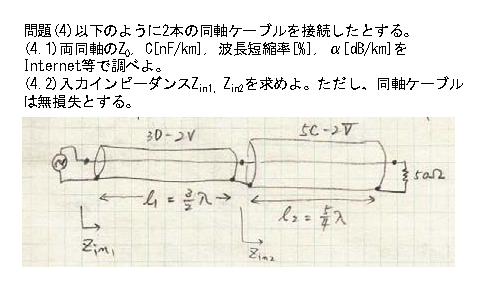
\includegraphics[width=140mm]{q4.png}
    \caption{問題}
    \label{p1}
  \end{center}
\end{figure}

\newpage

\section{解答}

図 \ref{sc1}のソースコードに解答例を示す.

\begin{figure}[H]
  \begin{center}
    \begin{screen}
      \begin{verbatim}
import numpy as np

def calculateInputImpedanceByFMatrix(Z0, Zr, cableLength):
  alpha = 0 # 無損失
  beta = 2 * np.pi
  gamma = alpha + beta * 1j
  theta = gamma * cableLength
  
  # 受信端にZrを接続した場合のf行列
  f_matrix = np.array([
    [np.cosh(theta) + Z0 * np.sinh(theta) / Zr,
    Z0 * np.sinh(theta)],
    [(np.sinh(theta) / Z0) + (np.cosh(theta) / Zr),
    np.cosh(theta)],
  ])
  
  return abs(f_matrix[0, 0] / f_matrix[1, 0])

Z02 = 75 # 同軸ケーブルのインピーダンス
Zr = 50 # 受端のインピーダンス

l2 = 5 / 4

Zin2 = calculateInputImpedanceByFMatrix(Z02, Zr, l2)

l1 = 3 / 2
Z01 = 50 # 同軸ケーブルのインピーダンス

Zin1 = calculateInputImpedanceByFMatrix(Z01, Zin2, l1)

print('Zin1 =', Zin1) # Zin1 = 112.5
print('Zin2 =', Zin2) # Zin2 = 112.5
\end{verbatim}
    \end{screen}
    \caption{ソースコード}
    \label{sc1}
  \end{center}
\end{figure}

また, 図 \ref{sc1}のソースコードにあるF行列は, 受信端に$Z_R$を接続した際のF行列である.
図 \ref{p2}に導出過程を示す.

\begin{figure}[H]
  \begin{center}
 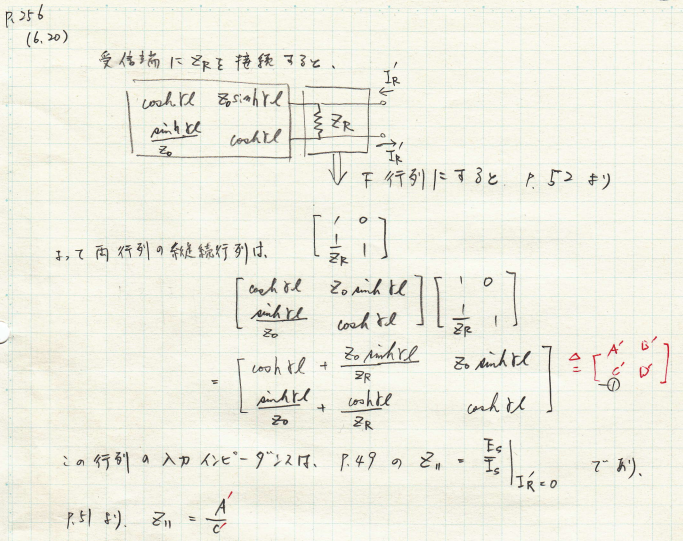
\includegraphics[width=160mm]{fmatrix.png}
 \caption{受信端に$Z_R$を接続した際のF行列の導出過程}
 \label{p2}
 \end{center}
 \end{figure}

\section{おわりに}

今回は同軸ケーブルの入力インピーダンスを求める問題をPythonを使って解いた.

\begin{thebibliography}{5}
  \bibitem{1}都築,”2020Q4-応用通信工学II-都築”,moodle内,参照 October 20,2021.
\end{thebibliography}

\end{document}